
\documentclass{article}
\usepackage[utf8]{inputenc} % 支持 UTF-8 编码
\usepackage{ctex}
\usepackage{xcolor}
\usepackage{tikz}
\usetikzlibrary{tikzmark}
\usepackage{amsmath}        % 数学公式支持
\usepackage{graphicx}       % 图片插入支持
\usepackage{geometry}       % 页面布局调整
\usepackage{lipsum}
\usepackage{tabularx}
\usepackage{xcolor} % 设置颜色
\usepackage{booktabs} % 提供美观的表格线条
\usepackage{array}    % 提供增强的列格式支持
\usepackage{multirow} % 支持多行合并单元格
\usepackage{makecell} % 支持单元格内容换行
%\usepackage[style=authoryear,backend=biber]{biblatex}
\usepackage{tikz}
\usepackage{array}
\usepackage{diagbox}
\usetikzlibrary{shapes,arrows.meta,positioning}
\usepackage[
colorlinks=true,          % 是否显示颜色而不是边框
linkcolor=blue,           % 内部链接颜色(如目录、交叉引用)
citecolor=red,            % 引用颜色
urlcolor=blue             % URL 颜色
]{hyperref}
\geometry{a4paper, margin=1in} % 设置页面边距


%\addbibresource{refs/references.bib} % 加载参考文献文件


\begin{document}
\pagenumbering{roman} % 设置页码为罗马数字
% 封面

% 封面页
\begin{titlepage}
	\centering

	% 校徽
	
\includegraphics[width=0.6\textwidth]{img/SZU_logo.png} \\
	\vspace{0.5cm} % 校徽与标题之间的间距
	
	% 标题
	\LARGE\bfseries
	综合论文题目: \\
	\vspace{0.5cm} % 标题与副标题之间的间距
	
	% 副标题
	\large\bfseries
	微波技术理论知识框架概括 \\
	\textit{(微波原理课程论文)} \\
	
	\vspace{2cm} % 副标题与正文信息之间的间距
	
	% 正文信息
	\begin{tabular}{l l}
		系别: & 计算机科学与技术系 \\
		专业: & 计算机科学与技术 \\
		学号: & 2025010426 \\
		姓名: & Carroll Polo \\
		指导教师: & Miller  \\
		副指导教师: & Aerith  \\
	\end{tabular}
	
	\vfill % 填充剩余空间到页面底部
	
	% 日期
	\large
	二〇二五年四月 \\
\end{titlepage}



	


%\maketitle

% 学位论文指导小组、公开评阅人和答辩委员会名单
% 本科生不需要
%\input{data/committee}

% 使用授权的说明
% 本科生开题报告不需要
%\copyrightpage
% 将签字扫描后授权文件 scan-copyright.pdf 替换原始页面
% \copyrightpage[file=scan-copyright.pdf]
%\frontmatter

% 中英文摘要和关键字
% 中文摘要
\renewcommand{\abstractname}{摘要} % 将 abstract 标题改为“摘要”
\begin{abstract}
微波原理课程是电子信息工程、通信工程及相关专业的重要基础课程,主要研究微波技术的基本理论和应用。本课程系统地介绍了微波的基本概念、特性及其在现代通信、雷达、遥感等领域的广泛应用。以下是该篇论文的具体结构划分。

第 1 章绪论介绍微波的基本概念和特性以及微波技术的发展和应用领域;第 2 章从“路”的观点出发,讲述传输线的基本理论,介绍反射系数、驻波比、输入阻抗、阻抗圆图和阻抗匹配等概念;第 3 章从“场”的观点出发,讲述波导、同轴线、带状线和微带线等典型微波传输线的一般理论和特性,给出常用的电磁波型、场分布和相应参数等;第 4 章采用“场”与“路”相结合的方法,讲述微波网络的基本理论,其中包括微波网络参量、网络矩阵和工作特性参量;第 5 章介绍各种常用微波元件的工作原理和应用。


\end{abstract}

% 中文关键词
\noindent \textbf{关键词:} 
微波原理,
传输线理论,
阻抗匹配,
微波网络,
微波元件,
波导,
同轴线,
带状线,
微带线,
电磁场分布,
网络矩阵,
工作特性参量
\addcontentsline{toc}{section}{摘要} % 将摘要添加到目录中

\; 

\renewcommand{\abstractname}{Abstract} % 恢复为默认的“Abstract”


\begin{abstract}
Microwave Principles is an essential foundational course for students in electronic information engineering, communication engineering, and related fields. It primarily focuses on the basic theories and applications of microwave technology. This course systematically introduces the fundamental concepts, characteristics, and widespread applications of microwaves in modern communications, radar, remote sensing, and other fields. The following is the specific structure of this paper.

Chapter 1 provides an introduction to the basic concepts and characteristics of microwaves, as well as the development and application areas of microwave technology. Chapter 2 discusses the basic theory of transmission lines from the perspective of "lines," introducing key concepts such as reflection coefficient, standing wave ratio, input impedance, Smith chart, and impedance matching. Chapter 3 explains the general theory and characteristics of typical microwave transmission lines, including waveguides, coaxial cables, strip lines, and microstrip lines, from the perspective of "fields." It also presents commonly used electromagnetic wave types, field distributions, and relevant parameters. Chapter 4 combines the perspectives of "fields" and "lines" to introduce the basic theory of microwave networks, covering microwave network parameters, network matrices, and operational characteristic parameters. Chapter 5 describes the working principles and applications of various common microwave components.


\end{abstract}

% 英文关键词
\noindent \textbf{Keywords:}
Microwave principle,
Transmission line theory,
Impedance matching,
Microwave network,
Microwave components,
Waveguide,
Coaxial line,
Strip line,
Microstrip line,
Electromagnetic field distribution,
Network matrix,
Operating characteristic parameters

\addcontentsline{toc}{section}{Abstract} % 将摘要添加到目录中

\newpage

\tableofcontents % 目录
%\addcontentsline{toc}{section}{abstract}
%\addcontentsline{toc}{section}{Abstract}

\clearpage % 强制开始新页,将目录与正文分开
% 插图和附表清单
% 本科生的插图索引和表格索引需要移至正文之后、参考文献前
% \listoffiguresandtables  % 插图和附表清单(仅限研究生)
%\listoffigures           % 插图清单
%\listoftables            % 附表清单
\pagenumbering{arabic} % 阿拉伯数字
% 符号对照表
%\input{data/denotation}


% 正文部分
%\mainmatter

\section{绪论/Introduction}

微波技术是 20 世纪初发展起来的,特别是第二次世界大战中雷达的研制加速了微波技术的发展,使其成为一门独立的学科。它主要研究的对象是微波。微波是一种频率非常高的电磁波,它在电磁波谱中占有很小的波段范围,如图 1 所示。

\begin{figure}[htbp]
	\centering
	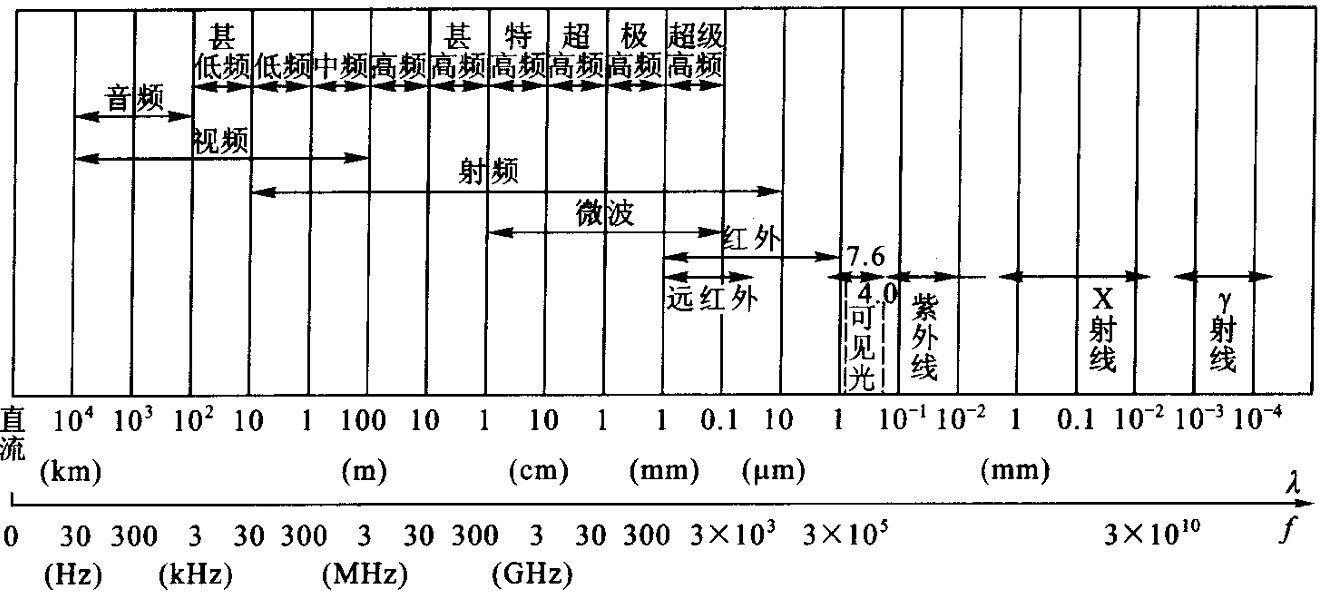
\includegraphics[width=0.8\textwidth]{img/1-1.png} % 图片文件名,不需要加扩展名
	\caption{微波频段示意图 \cite{chen2019artificial}}
	\label{fig:example}
\end{figure}

微波的定义:把波长在 1m - 0.1mm 范围内的电磁波称为微波。微波波段对应的频率范围为:
\( 3 \times 10^8 \sim 3 \times 10^{12} \, \text{Hz} \)
。在整个电磁波谱中,微波处于普通无线电波与红外线之间(包含了远红外部分),是频率最高的无线电波,它的频带宽度比所有普通无线电波波段总和宽约 10000 倍。一般情况下,微波又可划分为分米波、厘米波、毫米波和亚毫米波四个波段。

\subsection{微波的特性}
与普通无线电波相比,微波具有如下四个主要特性。

1.似光性

微波波长短,它的波长比地球上的宏观物体(如建筑物、飞机和军舰等)的尺寸小得多,其传播特性与光相似:沿直线传播、遇到障碍物时会产生反射。利用这一特点,可以制造出高方向性微波天线,用来发射或接收微波信号。从而为雷达、微波中继通信、卫星通信和导弹制导等提供了必要条件。

2.频率高

与普通无线电波相比,微波的频率要高得多,在同样的相对带宽条件下,微波的可用绝对带宽特别宽,能容纳的信息容量很大。因此,微波可作为多路通信的载频。另外,微波受外界干扰小、且不受电离层变化的影响,故通信质量高于普通无线电波。

由于微波的频率高,其振荡周期(10 −9 ∼10 −12s)与低频器件电子的渡越时间(一般为 10 −9s)属同一个数量级。因此,低频波段时可以忽略的一些物理现象,如极间电容、引线电感、集肤效应和辐射效应等,在微波波段特别明显,必须加以考虑。此外,传输微波的电路是一种分布参数电路,所使用的器件是特殊的微波器件。

3.能穿透电离层

利用本身的高频振荡,微波可以穿透电离层。由于微波不能被电离层所反射,所以微波的地面通信只限于天线的视距范围之内,远距离微波通信需要用中继站接力。但另一方面,利用微波能穿透电离层这一特点,又可以进行宇航通信、卫星通信和射电天文学研究等,因此微波开辟了电磁波谱中的一个“宇宙窗口”。

4.量子特性

微波具有波粒二象性。根据量子学理论,电磁辐射的能量不是连续的,而是由一个个的“能量子”组成,每个量子具有与其频率成正比的能量 E = hf)(其中 (f 为频率,普朗克常数 h=6.626×10 −34
J·s)。低频无线电波的频率很低,量子能量甚小,故其量子特性不明显。而微波的频率很高,其量子能量范围大约在 10 −5∼10 −2eV,故在低功率电平下,微波的量子特性明显地表现出来。另外,一些分子和原子的超精细结构能级落在微波波段,顺磁物质在磁场作用下的能级差也落在这一波段。利用微波与这些物质相互作用产生的物理现象,可用以研究物质的结构,从而形成一门“微波波谱学”。微波与物质的相互作用比较强烈,特别是水分子吸收了微波能量后会产生热效应,这一特点在实际中可以充分利用。

\subsection{微波技术的研究方法}
微波技术的基本理论是经典的电磁场理论,研究电磁波沿传输线的传播特性有两种分析方法。一种是“场”的分析方法,即从麦克斯韦方程出发,在特定边界条件下解电磁波动方程,求得场量的时空变化规律,分析电磁波沿线的各种传输特性;另一种是“路”的分析方法,即将传输线作为分布参数电路处理,用基尔霍夫定律建立传输线方程,求得线上电压和电流的时空变化规律,分析电压和电流的各种传输特性。事实上,“场”和“路”的分析方法是紧密相关的,很多方面两者相互补充。

因为在微波领域中所有的电磁现象都是随时间和空间而变化的物理过程,有的宜用“路”的方法处理,因此电路理论中的许多概念和方法在这里同样具有重要的地位。另一些电磁现象却宜用“场”的方法。有时对同一电磁现象既可用“路”的方法,也可用“场”的方法,两种方法只是分析同一问题的不同途径。

\subsection{微波技术的应用}
微波技术的实际应用相当广泛,尤其近年来随着它的发展,新的应用层出不穷。这里简单介绍几种主要应用。

1.在雷达方面的应用

雷达是微波技术的早期应用,事实上,正是由于第二次世界大战期间对于雷达的需要,微波技术才迅速发展起来。雷达设备可以利用微波信号准确地测定目标的方向、距离和速度,从而对运动目标实现定位、跟踪和识别。目前,用于军事上的有制导雷达、跟踪雷达、警戒雷达和炮瞄雷达等;用于民用上的有导航雷达、气象雷达和遥感雷达等。

2.在通信方面的应用

由于微波频带宽,信息容量大,因此微波可用于多路通信。在有线通信方面,利用同轴电缆可以同时传送几千路电话和几路电视信号;在无线通信方面,利用微波的中继接力传送电视信号,利用微波能穿透电离层的特性,可进行卫星通信和宇航通信,利用外层空间三颗互成 120 ∘角的同步卫星,就能实现全球通信和电视实况转播。

3.医学与生物工程

微波治疗:微波被用于肿瘤治疗(如微波消融术)和皮肤病的治疗。
生物传感:微波技术用于检测生物组织的电磁特性,帮助诊断疾病。
药物合成:微波辅助化学反应加速药物合成过程。




\section{传输线理论}

凡是能够导引电磁波沿一定方向传输的导体、介质系统均可称为传输线。微波传输线不仅可以用来传输电磁能量,还可用来构成各种微波元件。微波传输线种类繁多,按其传输的电磁波波型,大致可划分为三种类型。

\subsection{微波的传播特性}

与射频一样,微波是非电离且非破坏性的,从本质上来说,对人类是安全的。微波是一种高频电磁波,其波长范围为 0.3 mm 至 300 mm(对应频率范围为 1 GHz 至 1 THz)。由于其波长较长,微波的穿透能力比可见光、紫外线或 X射线强,但比低频无线电波弱。微波无线电P传播的路径损耗(Lp)是无线通信和成像的一个主要参数,由Friis公式\cite{huang2021antennas}控制

\begin{equation}
	L_{\mathrm{p}} = 10 \times \lg \left( \frac{P^{\mathrm{t}}}{P^{\mathrm{r}}} \right) = 20 \times \lg f + 20 \times \lg r - 147.6 \ (\text{in dB})
	\tag{1}
\end{equation}



其中,Pt是发射器功率;Pr是接收器功率;f是频率;r是距离。我们可以看出,路径损耗与频率f的平方和距离r的平方成正
比。频率越高,路径损耗就越大。


\subsection{传输线及其方程的解}

传输线方程是研究传输线上电压、电流的变化规律及其相互关系的方程。它可由均匀传输线的等效电路导出。

\begin{figure}[htbp]
	\centering
	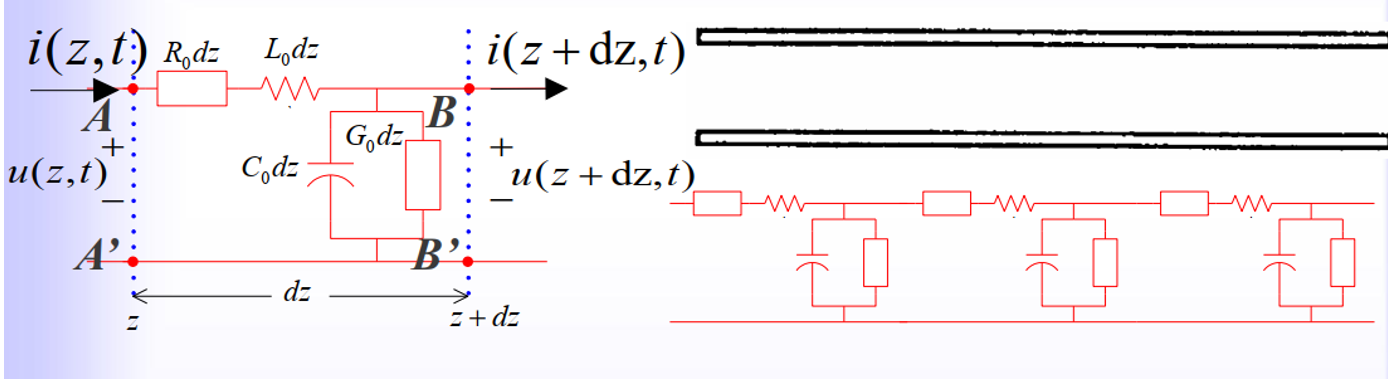
\includegraphics[width=0.8\linewidth]{img/2-1.png}
	\caption{传输线等效电路图}
	\label{fig:2-1}
\end{figure}

对于均匀传输线,取一个微元段 \( \mathrm{d}z \),其集中参数分别为 \( R_0 \, \mathrm{d}z \)、\( G_0 \, \mathrm{d}z \)、\( L_0 \, \mathrm{d}z \) 及 \( C_0 \, \mathrm{d}z \)。

等效电路如图 2 所示。传输线的始端接角频率为 ω 的正弦信号源,终端接负载阻抗 Z 
L。坐标原点选在始端。设距始端 z 处的电压和电流分别为 u 和 i,经过 dz 段后电压和电流分别为 u−du 和 i−di。传输线上的电压 u 和电流 i 既是位置坐标 z 的函数又是时间 t 的函数,可分别表示为 u=u(z,t),i=i(z,t)。经过 dz 段后电压和电流的变化量为


\begin{equation}
	\begin{cases}
		\displaystyle \frac{u(z + \mathrm{d}z, t) - u(z, t)}{\mathrm{d}z} = -R_0 \cdot i(z, t) - L_0 \cdot \frac{\partial i(z, t)}{\partial t} \\[12pt]
		\displaystyle \frac{i(z + \mathrm{d}z, t) - i(z, t)}{\mathrm{d}z} = -G_0 \cdot u(z + \mathrm{d}z, t) - C_0 \cdot \frac{\partial u(z + \mathrm{d}z, t)}{\partial t}
	\end{cases}
	\tag{2}
\end{equation}


\begin{equation}
	\begin{aligned}
		& \left\{
		\begin{aligned}
			\frac{\partial u(z, t)}{\partial z} &= -R_0 \cdot i(z, t) - L_0 \cdot \frac{\partial i(z, t)}{\partial t} \\
			\frac{\partial i(z, t)}{\partial z} &= -G_0 \cdot u(z, t) - C_0 \cdot \frac{\partial u(z, t)}{\partial t}
		\end{aligned}
		\right. \\
		& \quad \text{\tikzmarknode{eq1}{}} \quad \text{\tikzmarknode{eq2}{}} \\
		& \left\{
		\begin{aligned}
			\frac{d^2 U(z)}{dz^2} - \gamma^2 U(z) &= 0 \\
			\frac{d^2 I(z)}{dz^2} - \gamma^2 I(z) &= 0
		\end{aligned}
		\right.
	\end{aligned}
	\tag{2-2-3}
\end{equation}

如上公式2-2-3所示,1为时域电报方程,2为频域电报方程。时域电报方程描述了传输线上电压 u(z,t) 和电流 i(z,t) 随位置 z 和时间 t 的变化规律。频域电报方程是时域电报方程的傅里叶变换形式,主要用于分析稳态正弦信号在传输线上的传播特性。

\begin{equation}
	\begin{aligned}
		& \left\{
		\begin{aligned}
			U(z) &= A_1 e^{-\gamma z} + A_2 e^{\gamma z} \\
			I(z) &= \frac{1}{Z_0} \big( A_1 e^{-\gamma z} - A_2 e^{\gamma z} \big)
		\end{aligned}
		\right. \\
		& \quad \text{\tikzmarknode{eq3}{}} \quad \text{\tikzmarknode{eq4}{}} \\
		& \left\{
		\begin{aligned}
			U(z) &= U_i(z) + U_r(z) = U_i(z) [1 + \Gamma(z)] \\
			I(z) &= I_i(z) + I_r(z) = I_i(z) [1 - \Gamma(z)]
		\end{aligned}
		\right.
	\end{aligned}
	\tag{2-2-4}
\end{equation}

这两个公式分别描述了传输线上的电压和电流分布,以及入射波与反射波的关系。公式1这组公式描述了传输线上电压 U(z) 和电流 I(z) 的分布。
z 表示沿传输线的位置坐标,从参考点(通常为传输线的始端)开始测量。
公式2这组公式描述了传输线上的总电压和总电流如何由入射波和反射波组成。
$U(z)$ 和 $I(z)$ 分别是总电压和总电流,而 $U_i(z)$、$U_r(z)$、$I_i(z)$、$I_r(z)$ 分别表示入射波和反射波的电压和电流分量。



\subsection{传输线的特性参量}
传输线的特性参数主要包括:传播常数、特性阻抗、相速和相波长、输入阻抗、反射系数、驻波比(行波系数)和传输功率等。下面以相对重要的传播参数和特性阻抗分别加以介绍。

\subsubsection{传播参数}

\[
\gamma = \sqrt{(R_0 + j \omega L_0)(G_0 + j \omega C_0)} = \alpha + j \beta
\]

- $\alpha$ 是衰减常数,表示行波每经过单位长度后振幅的衰减倍数,其单位为分贝/米 (dB/m) 或奈培/米 (Np/m);
- $\beta$ 是相位常数,表示行波每经过单位长度后相位滞后的弧度数,单位为弧度/米 (rad/m)。

\[
\gamma = j \omega \sqrt{L_0 C_0} = j \beta \quad (\beta = \omega \sqrt{L_0 C_0})
\]

\subsubsection{特性阻抗}

\[
Z_0 = \frac{U_i}{I_i} = -\frac{U_r}{I_r} \quad (\text{定义})
\]
\[
Z_0 = \sqrt{\frac{Z}{Y}} = \sqrt{\frac{R_0 + j \omega L_0}{G_0 + j \omega C_0}}
\]
\[
Z_0 = \sqrt{\frac{L_0}{C_0}} \quad (\text{无耗传输线})
\]

\subsubsection{相位关系与波速}

\[
\text{Pha.} = \omega t - \beta z = \text{Constant}
\]
两边求导:
\[
v_p = \frac{dz}{dt} = \frac{\omega}{\beta} \quad (\text{时域解})
\]

上式均适用有耗/无耗传输线。

\subsubsection{波长与频率的关系}

\[
\lambda_p = \frac{v_p}{f} = \frac{2\pi}{\beta}
\]


\subsection{阻抗圆图及应用}
在微波工程中,经常会遇到输入阻抗、负载阻抗、反射系数和驻波比等参数的计算问题;此外,还有阻抗匹配方面的问题。若用前面介绍的公式计算,会遇到大量的复数运算,非常繁琐。工程上常用阻抗圆图来分析和计算,既方便又直观,而且具有一定精度,可满足工程设计要求,因而圆图作为处理微波传输线问题的一种图解法,在实际中获得了普遍应用。

下面介绍圆图的构造、原理及其应用。为了使阻抗圆图适用于任意特性阻抗的传输线的计算,故圆图上的阻抗均采用归一化阻抗。

\begin{figure}[htbp]
	\centering
	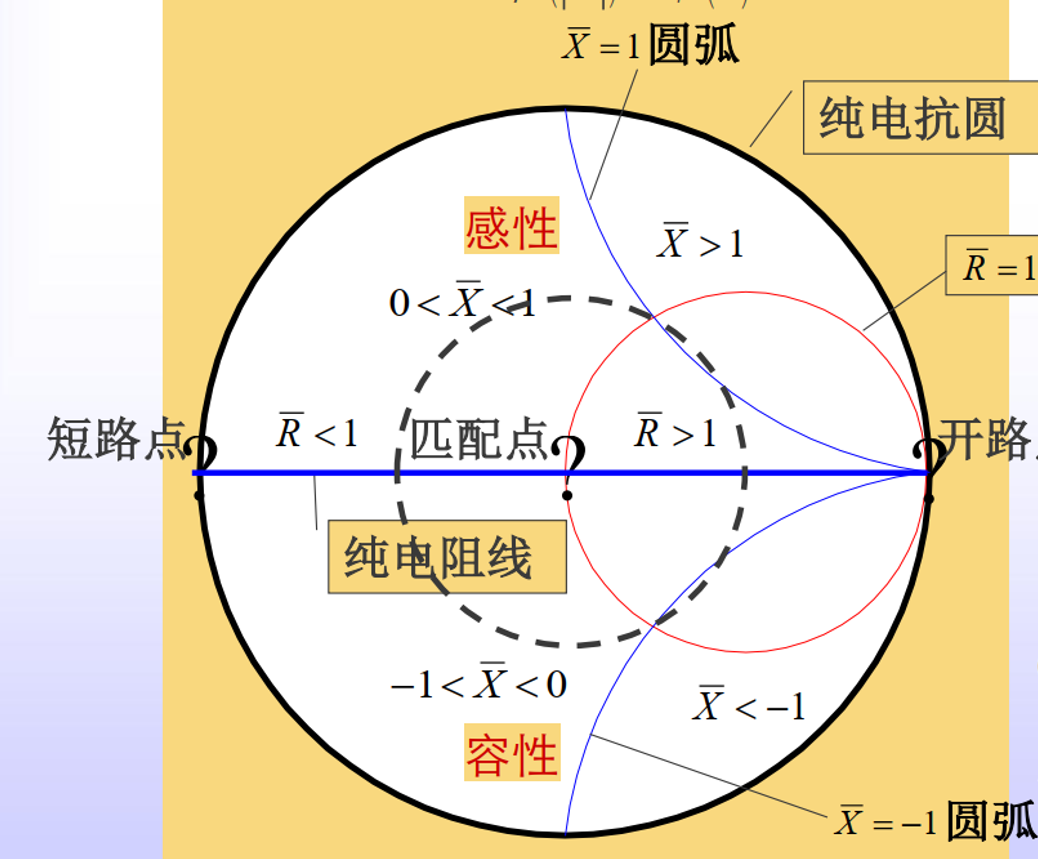
\includegraphics[width=0.5\linewidth]{img/2-4}
	\caption{阻抗圆图及其重要的点线面}
	\label{fig:2-4}
\end{figure}

(1) 三个圆族:反射系数圆;等电阻圆;等电抗圆。

(2) 三个特殊点:
开路点;匹配点;短路点。

(3) 三条特殊线:
纯电阻线;纯电抗圆;可匹配圆(串联)。

(4) 二个特殊面:
上半圆平面(感性)和下半圆平面(容性)。

(5) 二个旋转方向:
“源顺负逆”。

\section{波导理论}

微波传输线是用来传输微波信号和微波能量的传输线。如第 2 章 2.1 节所介绍的那样,微波传输线的种类很多,比较常用的有平行双线、矩形波导、圆波导、同轴线、带状线和微带线等。一般根据不同的用途和工作频段选用不同类型的传输线。

在微波的低频段,可采用平行双线来传输微波电磁能量;但当频率提高后,平行双线会向空间辐射电磁能量,且频率愈高,能量损耗愈大。所以在微波的高频段,平行双线不能使用,一般采用同轴线和波导等类型的传输线,这类传输线是封闭式的,不存在辐射损耗。随着频率的继续提高,同轴线的横截面尺寸必须相应减小才能保证只传输 TEM 波,这样导致同轴线的导体损耗增加,功率容量下降。因此同轴线不能传输更高频率的电磁波,一般只适用于厘米波段。

对于更高频率的电磁波,可采用波导进行传输。波导是空心金属管,它传输的功率容量最大;但它的带宽较窄,体积和重量较大。随着空间技术的发展,对微波集成电路需要越来越多,显然同轴线和波导不能满足这种需要,所以出现了带状线和微带线等形式的传输线。特别是微带线,具有体积小、重量轻和频带宽等优点,是目前微波集成电路中采用最多的传输线。但它的缺点是功率容量小,损耗较大,所以主要用于小功率系统中。

微波传输线是引导电磁波沿一定方向传输的系统,故又称做导波系统。被传输的电磁波又称做导行波。导行波一方面要满足麦克斯韦方程,另一方面又要满足导体或介质的边界条件;也就是说,麦克斯韦方程和边界条件决定了导行波在导波系统中的电磁场分布规律和传播特性。

本章首先采用电磁场理论来分析矩形波导、圆波导和同轴线的传播特性和电磁场分布规律,然后借助传输线理论来分析带状线、微带线、耦合带状线和耦合微带线的基本特点和传输规律。



\subsection{交变电磁场基本关系式}

\textbf{场量的瞬时值与复数振幅值之间的关系为}
\[
E(x, y, z, t) = E(x, y, z) \cos(\omega t + \theta)
\]
\[
= \operatorname{Re}\left[\underline{E}(x, y, z) e^{j\theta} e^{j\omega t}\right] = \operatorname{Re}\left[\hat{E}(x, y, z) e^{j\omega t}\right]
\tag{3-1-1}
\]

\textbf{可得复数形式的麦克斯韦方程组为}
\[
\begin{aligned}
	\nabla \times \dot{E} &= -j \omega \mu \dot{H}, \\
	D &= \varepsilon E, \\
	B &= \mu H, \\
	\nabla \times \dot{H} &= j \omega \varepsilon \dot{E} + J, \\
	\nabla \cdot \dot{D} &= \rho, \\
	\nabla \cdot \dot{B} &= 0
\end{aligned}
\tag{3-1-2}
\]

一般都假定远离场源 $\rho = 0$, $J = 0$,即在无源区
\[
\begin{aligned}
	\nabla \times E &= -j \omega \mu H, \\
	\nabla \times H &= j \omega \varepsilon E, \\
	\nabla \cdot D &= 0, \\
	\nabla \cdot B &= 0.
\end{aligned}
\tag{3-1-3}
\]

\subsection{边界条件}

\begin{figure}[htbp]
	\centering
	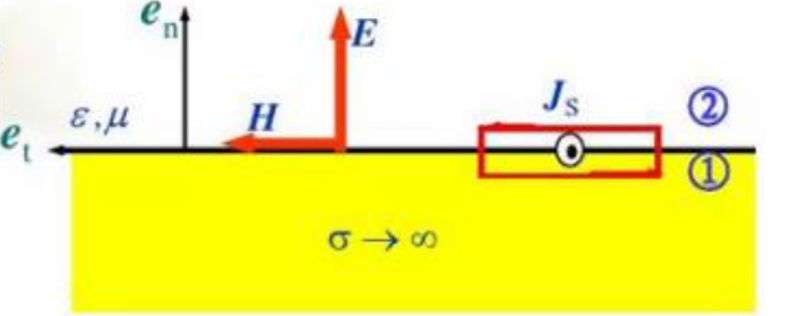
\includegraphics[width=0.4\textwidth]{img/3-5.png} % 图片文件名,不需要加扩展名
	\caption{边界条件示意图}
	\label{fig:example}
\end{figure}

\begin{equation}
	\begin{aligned}
		n \times (E_2 - E_1) &= 0 & \quad (E_{2t} - E_{1t}) &= 0 \\
		n \times (H_2 - H_1) &= J_s & \quad (H_{2t} - H_{1t}) &= 0 \\
		n \cdot (D_2 - D_1) &= \rho_s & \quad (D_{2n} - D_{1n}) &= 0 \\
		n \cdot (B_2 - B_1) &= 0 & \quad (B_{2n} - B_{1n}) &= 0
	\end{aligned}
	\tag{3-2-1}
\end{equation}

式中 $ n $ 为由媒质 1 指向媒质 2 的法向单位矢量,$ J_s $ 为界面上的电流密度,$ \rho_s $ 为界面上的面电荷密度。
$ n $:由媒质 1 指向媒质 2 的法向单位矢量;
$ J_s $:界面上的电流密度;
$ \rho_s $:界面上的面电荷密度。

在理想导体表面上,电场 $E_2$​总是垂直于表面,而磁场$ H_2​$总是平行于表面;电位移矢量 $D 2​$等于自由电荷面密度$ ρ s​$,并垂直于表面;在导体表面上的电流密度 $J s$等于表面的磁场强度$ H 2​$,其方向为 $n$× $H 2$ ,并可由右手定则确定。


\subsection{理想波导系统的一般理论}

理想导波系统一般指规则的金属波导管,分析时一般只讨论远离场源的区域,并常采用广义正交坐标系 $(u_1, u_2, z)$,其中 $u_1$ 和 $u_2$ 为波导横截面上的坐标,$z$ 为波导纵向坐标。导波系统中电场和磁场在广义正交坐标系中,可用其横向分量和纵向分量来表示
\begin{align*}
	\mathbf{E}(u_1, u_2, z) &= \mathbf{E}_T(u_1, u_2, z) + \mathbf{E}_z(u_1, u_2, z) = \mathbf{E}_T + \mathbf{E}_z 
	\tag{3-3-1}
	\\
	\mathbf{H}(u_1, u_2, z) &= \mathbf{H}_T(u_1, u_2, z) + \mathbf{H}_z(u_1, u_2, z) = \mathbf{H}_T + \mathbf{H}_z
	\tag{3-3-2}
\end{align*}
式中:$\mathbf{E}_T$ 和 $\mathbf{H}_T$——电场和磁场的横向分量;\\
$\mathbf{E}_z$ 和 $\mathbf{H}_z$——电场和磁场的纵向分量。

导波系统中的电磁波按纵向场分量的有无,可分为以下三种波型(或模):
\begin{enumerate}
	\item 横磁波(TM 波),又称电波(E 波):$\mathbf{H}_z = 0$, $\mathbf{E}_z \neq 0$;
	\item 横电波(TE 波),又称磁波(H 波):$\mathbf{E}_z = 0$, $\mathbf{H}_z \neq 0$;
	\item 横电磁波(TEM 波):$\mathbf{E}_z = 0$, $\mathbf{H}_z = 0$。
\end{enumerate}

其中横电磁波只存在于多导体系统中,它是非色散波;而横磁波和横电波一般存在于单导体系统中,它们是色散波。下面分别讨论上述三种波型的场量关系式。


\begin{table}[htbp]
	\centering
	\caption{三类波型的主要关系式}
	\label{tab:wave_relations}
	\begin{tabular}{c|c|c|c}
		\hline
		& TEM 波 & TM 波 & TE 波 \\
		\hline
		横向分布函数 & 拉普拉斯方程 & 亥姆霍兹方程 & 亥姆霍兹方程 \\
		& $\nabla^2 \phi = 0$ & $\nabla^2 \phi + k_c^2 \phi = 0$ & $\nabla^2 \psi + k_c^2 \psi = 0$ \\
		\hline
		相移常数 ($k > k_c$) & $\beta = k = \omega \sqrt{\mu \epsilon}$ & $\beta = \sqrt{k^2 - k_c^2}$ & $\beta = \sqrt{k^2 - k_c^2}$ \\
		& & $k = \omega \sqrt{\mu \epsilon}$ & $k = \omega \sqrt{\mu \epsilon}$ \\
		\hline
		广义传输线方程 & $\frac{\mathrm{d}U(z)}{\mathrm{d}z} = -j \omega \mu I(z)$ & $\frac{\mathrm{d}U(z)}{\mathrm{d}z} = \frac{1}{j \omega \epsilon} (k^2 - k_c^2) I(z)$ & $\frac{\mathrm{d}I(z)}{\mathrm{d}z} = -j \omega \mu U(z)$ \\
		& $\frac{\mathrm{d}I(z)}{\mathrm{d}z} = -j \omega \epsilon U(z)$ & $\frac{\mathrm{d}I(z)}{\mathrm{d}z} = -j \omega \epsilon U(z)$ & $\frac{\mathrm{d}I(z)}{\mathrm{d}z} = \frac{1}{j \omega \mu} (k^2 - k_c^2) U(z)$ \\
		\hline
		纵向场分量 & $E_z = H_z = 0$ & $E_z = \boldsymbol{\alpha}_z \frac{I(z)}{j \omega \epsilon} k_c^2 \phi$ & $H_z = \boldsymbol{\alpha}_z \frac{U(z)}{j \omega \mu} k_c^2 \psi$ \\
		\hline
		横向场分量 & $E_T = -U(z) \nabla_T \phi$ & $E_T = -U(z) \nabla_T \phi \times \boldsymbol{\alpha}_z$ & $E_T = -U(z) \nabla_T \psi \times \boldsymbol{\alpha}_z$ \\
		& $H_T = I(z) \nabla_T \phi \times \boldsymbol{\alpha}_z$ & $H_T = I(z) \nabla_T \phi \times \boldsymbol{\alpha}_z$ & $H_T = I(z) \nabla_T \psi$ \\
		\hline
		波阻抗 & $Z_{\text{TEM}} = \eta = \sqrt{\frac{\mu}{\epsilon}}$ & $Z_{\text{TM}} = \frac{\beta}{\omega \epsilon} = \frac{\sqrt{\omega^2 \mu \epsilon - k_c^2}}{\omega \epsilon}$ & $Z_{\text{TE}} = \frac{\omega \mu}{\beta} = \frac{\omega \mu}{\sqrt{\omega^2 \mu \epsilon - k_c^2}}$ \\
		\hline
	\end{tabular}
\end{table}

\subsection{导波系统的传输特性}

1. “高通低不通”
→ 高通滤波器

2. 多模
理论上,在矩形波导中能存在着无穷多个 $TE_{mn} $、$ TM_{mn} $模式,它们都满足波动方程并能满足矩形波导的边界条件。

3. 主模
在波导中,通常称截止波长最大(对应截止波数或截止频率最小)的模式为主模,也称基模或最低模式。而将其他为实现单一 TE 10​模传输,必须满足下列条件:
\[
(\lambda_c)_{H_{10}} = 2a > \lambda > \max \left\{ (\lambda_c)_{H_{20}} = a, (\lambda_c)_{H_{01}} = 2b \right\}
\tag{3-4}
\]
4. 简并截止波数$ ( k_c )$或截止波长 $( \lambda_c )$、截止频率 $( f_c )$相同但场分布不同的模式称为“简并”模式。

5. 色散
相速度随频率变化的现象称为色散。

6. 完备性
由三角函数的完备性,可以证明,矩形波导中所有可能存在的导波场结构都可以用 $TE_{mn} $、$ TM_{mn} $模的线性组合来表示。

\subsection{矩形波导中电磁波型的传输特性}
虽然矩形波导中可能存在无限多的 TE 和 TM 波型,但哪些波型能够在波导中传输,还取决于工作频率和波导尺寸。合理地选择工作频率和波导尺寸,可以使需要的波型能传输,而使不需要的波型截止掉。


截止波长不仅与波导尺寸 a 和 b 有关,而且与决定波型的 m 和 n 有关。不同的 m 、n 值代表不同的波型,具有不同的场分布;但对同一组 m 、 n 值,TE 波和 TM 波有相同的截止波长(频率),即 (λ c​) TM mn​=(λ c​) TE mn​。这种截止波长(频率)相同而场分布不同的一对波型称为“简并波”。矩形波导中的波型一般都是简并的波型,但 TE m0
​和 TE 0n​是非简并波,因为矩形波导中不存在 TM m0​波和 TM 0n​波。

当波导尺寸 a 和 b 给定时,将不同 m 和 n 值代入式 (3-5-12a) 中,即可得到不同波型的截止波长。例如,对于常用 BJ-100 型波导,其标称尺寸为 a×b=22.86mm×10.16mm,故可计算出各波型的 λ c​值,其分布如图 3-5-2 所示。



\begin{figure}[htbp]
	\centering
	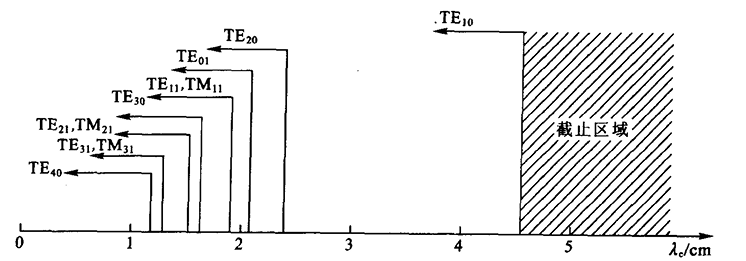
\includegraphics[width=0.7\linewidth]{img/3-6}
	\caption{识别文字BJ-100型波导不同波型截止波长的分布图}
	\label{fig:3-6}
\end{figure}

从图中可以看出,TE({10})模的截止波长最长,它右边的阴影区为截止区。

(1) 当工作波长 λ=5 cm 时,波导对所有的波型都截止,此时的波导称为“截止波导”。

(2) 当 λ=4 cm 时,波导只能传输 TE 10​
模,此时的波导称为“单模波导”。

(3) 当 λ=1.5 cm 时,波导可同时传输 $TE_{10}$、$TE_{20}$、$TE_{01}$、$TE_{11} $、$TM_{11}$ 及 $TE_{30}$等波型,此时的波导称为“多模波导”。

\subsection{圆波导中的三种主要模式}
圆波导中有无限多个模式存在,最常用的三个主要模式为 $TE_{11} $、$ TE_{01}$ 和 $TM_{01}$模。下面分别介绍这三种模式的特点和它们的应用。

\subsubsection{TE 11模 (λc= 3.41R)}

TE 11​模的场分布如图 6 所示。其中图 6(a) 表示横截面上的电磁场分布;图 6(b) 表示纵剖面上的电场分布;图 6(c) 表示圆波导壁上的壁电流分布。

\begin{figure}[htbp]
	\centering
	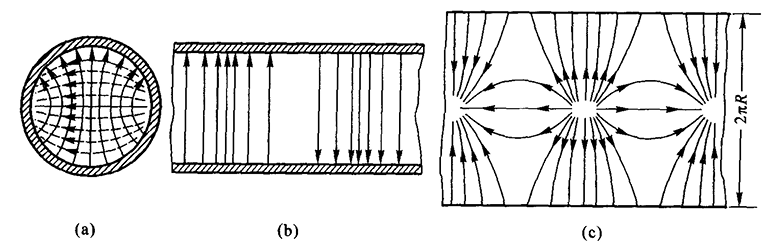
\includegraphics[width=0.7\linewidth]{img/3-6-1}
	\caption{$TE_{11}$模场分布图}
	\label{fig:3-6-1}
\end{figure}

由图可见,圆波导中 TE 11​模的场分布和矩形波导中 TE 10​模的场分布很相似,因此圆波导中 TE 11​模很容易通过矩形波导中 TE 10​模过渡得到,而且 TE 11​模的截止波长最长,容易实现单模传输。因此,圆波导的极化衰减器、波型变换器和铁氧体环行器均采用 TE 11​模作为工作模式。但由于 TE 11​模存在极化简并模,故不宜用来作为远距离传输的工作模式。

\subsubsection{ $TE_{01}$模 (λc=1.64R)}

$TE_{01}$模的场分布如图 7 所示。其中图 7(a) 表示横截面上的电磁场分布;图 7(b) 表示纵剖面上的电磁场分布;图 7(c) 表示壁电流分布。

\begin{figure}[htbp]
	\centering
	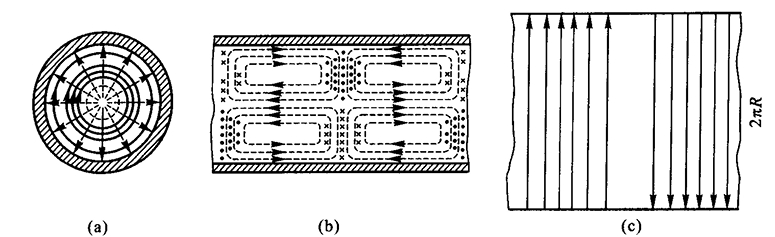
\includegraphics[width=0.7\linewidth]{img/3-6-2}
	\caption{$TE_{01}$模场分布图}
	\label{fig:3-6-2}
\end{figure}

由图可见,TE 01​模的电场只存在 E φ​分量,且在 r=0 和 R 处,$ E_varphi = 0 $;在波导壁上只有磁场的  $H_z$ 分量,故在壁上只有 J φ电流,且随频率的升高而减小,从而 TE 01​模的导体损耗随频率升高而降低。因此,TE 01模常作为高 Q 谐振腔和远距离的毫米波传输线的工作模式。另外由于它是圆电模,也可作为连接元件和天线馈线系统的工作模式。但由于它不是主模,因此该模式作为工作模式时,必须设法抑制其他模式。

\subsubsection{ $TM_{01}$模 (λc=1.64R)} 
TM 01模的场分布如图 8 所示。其中图 8(a) 表示横截面上的电磁场分布;图 8(b) 表示纵剖面上的电磁场分布;图 8(c) 表示壁电流的分布。

\begin{figure}[htbp]
	\centering
	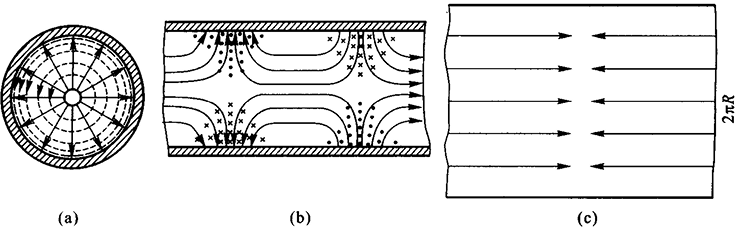
\includegraphics[width=0.7\linewidth]{img/3-6-3}
	\caption{$TM_{01}$模场分布图}
	\label{fig:3-6-3}
\end{figure}

由图可见,TM 01​模的磁场只有 H φ​分量,是具有轴对称分布的圆磁场;电场只有 E z分量,且在 r=0 处 E z​最大;壁电流只有纵向分量 J z​。因此适用于微波天线馈线旋转铰链的工作模式。由于它具有 E z分量,便于和电子交换能量,可做电子直线加速器的工作模式。但由于它的管壁电流具有纵向电流,故必须采用抗流结构的连接方式。







\section{微波网络理论}

任何一个微波系统都是由各种微波元件和微波传输线组成的。微波传输线的特性可以用广义传输线方程来描述,微波元件的特性可以用类似于低频网络的等效电路来描述。因此,任何一个复杂的微波系统都可以用电磁场理论和低频网络理论相结合的方法来分析,这种理论称为微波网络理论。

\subsection{二端口微波网络的网络参量}

在各种微波网络中,二端口微波网络是最基本的。例如,衰减器、移相器、阻抗变换器和滤波器等均属于二端口微波网络。对于一个线性二端口微波网络,应用叠加定理,可以得到表征网络特性的线性方程组。

表征二端口微波网络的参数可以分为两大类:一类是反映网络参考面上电压与电流之间关系的参数,对于图 4-4-1 中的二端口微波网络,参考面 T 1​和 T 2​上的电压和电流方向如图 4-4-1(a) 所示。另一类是反映网络参考面上入射波电压与反射波电压之间关系的参数,如图 4-4-1(b) 所示。

\begin{figure}
	\centering
	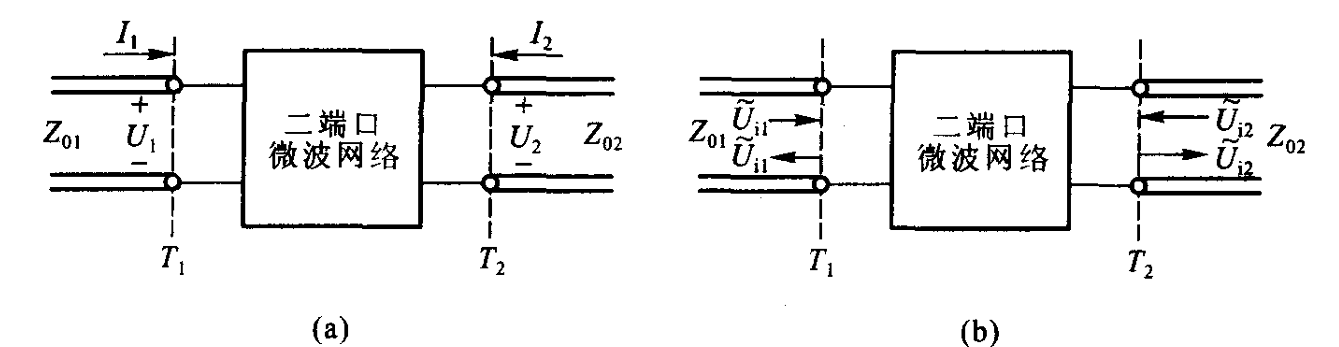
\includegraphics[width=0.7\linewidth]{img/4-3}
	\caption{二端口微波网络}
	\label{fig:4-3}
\end{figure}

如图 4-4-1(a) 所示的二端口微波网络,参考面 \( T_1 \) 和 \( T_2 \) 选在远离不均匀区,故不需要考虑高次模的影响。应用叠加定理可以写出两个参考面上电压与电流之间三种不同组合关系的线性方程组,从而可以得到三个网络参量。

(1) 阻抗参量

用 \( T_1 \) 和 \( T_2 \) 两个参考面上的电流表示两个参考面上的电压,其网络方程为:
\begin{equation}
	\begin{aligned}
		U_1 &= Z_{11} I_1 + Z_{12} I_2, \\
		U_2 &= Z_{21} I_1 + Z_{22} I_2.
	\end{aligned}
	\tag{4-4-1a}
\end{equation}
或写成矩阵形式为:
\begin{equation}
	\begin{bmatrix}
		U_1 \\
		U_2
	\end{bmatrix}
	=
	\begin{bmatrix}
		Z_{11} & Z_{12} \\
		Z_{21} & Z_{22}
	\end{bmatrix}
	\begin{bmatrix}
		I_1 \\
		I_2
	\end{bmatrix}.
	\tag{4-4-1b}
\end{equation}

(2) 导纳参量

用 $ T_1 $ 和 $ T_2 $ 两个参考面上的电压表示两个参考面上的电流,其网络方程为:
\begin{equation}
	\begin{aligned}
		I_1 &= Y_{11} U_1 + Y_{12} U_2, \\
		I_2 &= Y_{21} U_1 + Y_{22} U_2.
	\end{aligned}
	\tag{4-4-5a}
\end{equation}

或写成矩阵形式为:
\begin{equation}
	\begin{bmatrix}
		I_1 \\
		I_2
	\end{bmatrix}
	=
	\begin{bmatrix}
		Y_{11} & Y_{12} \\
		Y_{21} & Y_{22}
	\end{bmatrix}
	\begin{bmatrix}
		U_1 \\
		U_2
	\end{bmatrix}.
	\tag{4-4-5b}
\end{equation}

(3) 转移参量

用 $ T_2 $ 面上的电压、电流来表示 $ T_1 $ 面上的电压和电流的网络方程,且规定电流流进网络为正方向,流出网络为负方向。则有:
\begin{equation}
	\begin{aligned}
		U_1 &= A_{11} U_2 - A_{12} I_2, \\
		I_1 &= A_{21} U_2 - A_{22} I_2.
	\end{aligned}
	\tag{4-4-7a}
\end{equation}

写成矩阵形式为:
\begin{equation}
	\begin{bmatrix}
		U_1 \\
		I_1
	\end{bmatrix}
	=
	\begin{bmatrix}
		A_{11} & A_{12} \\
		A_{21} & A_{22}
	\end{bmatrix}
	\begin{bmatrix}
		U_2 \\
		-I_2
	\end{bmatrix}.
	\tag{4-4-7b}
\end{equation}

或简记为:
\[
\mathbf{A} =
\begin{bmatrix}
	A_{11} & A_{12} \\
	A_{21} & A_{22}
\end{bmatrix}.
\]

(4) 散射参量

二端口网络参考面 $ T_1 $ 和 $ T_2 $ 上的归一化入射波电压和归一化反射波电压的方向如图 4-4-1(b) 所示。应用叠加定理,可以用两个参考面上的入射波电压来表示两个参考面上的反射波电压,其方程为:
\begin{equation}
	\begin{aligned}
		\widetilde{U}_{r1} &= S_{11} \widetilde{U}_{i1} + S_{12} \widetilde{U}_{i2}, \\
		\widetilde{U}_{r2} &= S_{21} \widetilde{U}_{i1} + S_{22} \widetilde{U}_{i2}.
	\end{aligned}
	\tag{4-4-9a}
\end{equation}
或写成矩阵形式为:
\begin{equation}
	\begin{bmatrix}
		\widetilde{U}_{r1} \\
		\widetilde{U}_{r2}
	\end{bmatrix}
	=
	\begin{bmatrix}
		S_{11} & S_{12} \\
		S_{21} & S_{22}
	\end{bmatrix}
	\begin{bmatrix}
		\widetilde{U}_{i1} \\
		\widetilde{U}_{i2}
	\end{bmatrix}.
	\tag{4-4-9b}
\end{equation}

简记为:
\[
\widetilde{\mathbf{U}}_r = \mathbf{S} \widetilde{\mathbf{U}}_i.
\]

式中:
\begin{tabular}{p{0.3\textwidth} p{0.6\textwidth}}
	$ \mathbf{S} $ & —— 网络的散射矩阵; \\
	$ S_{11} $, $ S_{12} $, $ S_{21} $, $ S_{22} $ & —— 网络的散射参量。
\end{tabular}

由式 (4-4-9a) 可导出散射参数的定义为:
\begin{align*}
	S_{11} &= \left. \frac{\widetilde{U}_r}{\widetilde{U}_i} \right|_{\widetilde{U}_2 = 0}, & \text{表示 } T_2 \text{ 面接匹配负载时,} T_1 \text{ 面上的电压反射系数;} \\
	S_{12} &= \left. \frac{\widetilde{U}_r}{\widetilde{U}_i} \right|_{\widetilde{U}_1 = 0}, & \text{表示 } T_1 \text{ 面接匹配负载时,} T_2 \text{ 面至 } T_1 \text{ 面的电压传输系数;} \\
	S_{21} &= \left. \frac{\widetilde{U}_r}{\widetilde{U}_i} \right|_{\widetilde{U}_2 = 0}, & \text{表示 } T_2 \text{ 面接匹配负载时,} T_1 \text{ 面至 } T_2 \text{ 面的电压传输系数;} \\
	S_{22} &= \left. \frac{\widetilde{U}_r}{\widetilde{U}_i} \right|_{\widetilde{U}_1 = 0}, & \text{表示 } T_1 \text{ 面接匹配负载时,} T_2 \text{ 面上的电压反射系数。}
\end{align*}

由此可见,用散射参量来表示网络的电压反射系数和传输系数是很方便的,因此它是微波网络中最常用的一种参量。

(5) 传输参量

如图 4-4-1(b) 所示,应用叠加定理,还可以用 $ T_2 $ 面上的电压入射波和反射波来表示 $ T_1 $ 面上的电压,其方程为:
\begin{equation}
	\begin{aligned}
		\widetilde{U}_{i1} &= T_{11} \widetilde{U}_{a} + T_{12} \widetilde{U}_{r}, \\
		\widetilde{U}_{d} &= T_{21} \widetilde{U}_{a} + T_{22} \widetilde{U}_{r}.
	\end{aligned}
	\tag{4-4-10a}
\end{equation}
或写成矩阵形式为:
\begin{equation}
	\begin{bmatrix}
		\widetilde{U}_{i1} \\
		\widetilde{U}_{d}
	\end{bmatrix}
	=
	\begin{bmatrix}
		T_{11} & T_{12} \\
		T_{21} & T_{22}
	\end{bmatrix}
	\begin{bmatrix}
		\widetilde{U}_{a} \\
		\widetilde{U}_{r}
	\end{bmatrix}.
	\tag{4-4-10b}
\end{equation}

简记为:
\[
\mathbf{T} =
\begin{bmatrix}
	T_{11} & T_{12} \\
	T_{21} & T_{22}
\end{bmatrix}.
\]

式中:
- $\mathbf{T}$ —— 网络的传输矩阵;
- $T_{11}$、$T_{12}$、$T_{21}$ 和 $T_{22}$ —— 网络的传输参量。

由式 (4-4-10a) 可导出网络参量 $T_{11}$ 的定义为:
\[
T_{11} = \left. \frac{\widetilde{U}_{i1}}{\widetilde{U}_{a}} \right|_{\widetilde{U}_{r} = 0}
\]
表示 $T_2$ 面接匹配负载时,$T_1$ 面至 $T_2$ 面的电压传输系数的倒数。其余参量没有直观的物理意义。

\subsection{二端口微波网络参量的性质}

一般情况下,二端口网络的五种网络参量均有四个独立参量,但当网络具有某种特性(如对称性或可逆性等)时,网络的独立参量个数将会减少。下面讨论网络参量的性质。

\subsection*{1. 可逆网络}
如前所述,可逆网络具有互易特性,即
\[
\begin{aligned}
	Z_{12} &= Z_{21}, \quad \text{或} \quad \widetilde{Z}_{12} = \widetilde{Z}_{21}, \\
	Y_{12} &= Y_{21}, \quad \text{或} \quad \widetilde{Y}_{12} = \widetilde{Y}_{21}.
\end{aligned}
\]
根据五种网络参量的转换公式不难得到其他几种网络参量的互易特性为:
\[
\begin{aligned}
	A_{11} A_{22} - A_{12} A_{21} &= 1, \quad \text{或} \quad \widetilde{A}_{11} \widetilde{A}_{22} - \widetilde{A}_{12} \widetilde{A}_{21} = 1, \\
	S_{12} &= S_{21}, \quad T_{11} T_{22} - T_{12} T_{21} = 1.
\end{aligned}
\]
由此可见,一个可逆二端口网络只有三个独立参量。

\subsection*{2. 对称网络}
如前所述,一个对称网络具有下列特性:
\[
Z_{11} = Z_{22}, \quad Y_{11} = Y_{22}.
\]
根据网络参量的转换公式,可以得到其他几种网络参量的对称性为:
\[
S_{11} = S_{22}, \quad T_{12} = -T_{21}, \quad A_{11} = A_{22} \quad (Z_{01} = Z_{02}).
\]
由此可见,一个对称二端口网络的两个参考面上的输入阻抗、输入导纳以及电压反射系数等参量一一对应相等。

\subsection*{3. 无耗网络}
由 4.3 节可知,无耗网络的阻抗和导纳参量均为纯虚数,即
\[
Z_i = j X_i, \quad Y_j = j B_j \quad (i, j = 1, 2).
\]
利用各种参量的转换公式,不难得出转移参量和传输参量的无耗特性为:\( A_{11} \) 和 \( A_{22} \) 为实数,\( A_{12} \) 和 \( A_{21} \) 为纯虚数,且有:
\[
T_{11} = T_{22}^*, \quad T_{12} = T_{21}^*.
\]
利用复功率定理和矩阵运算可以证明,一个无耗网络的散射矩阵一定满足“么正性”,即式中:
- $ S^T $ —— $ S $ 的转置矩阵;
- $ S^* $ —— $ S $ 的共轭矩阵;
- $ 1 $ —— 单位矩阵。

若网络可逆,则有 $ S^T = S $,故对于无耗可逆二端口网络的散射参量具有下列的“一元性”,即
\[
S S^* = 1
\]
或写成
\[
\begin{bmatrix}
	S_{11} & S_{12} \\
	S_{21} & S_{22}
\end{bmatrix}
\begin{bmatrix}
	S_{11}^* & S_{21}^* \\
	S_{12}^* & S_{22}^*
\end{bmatrix}
=
\begin{bmatrix}
	1 & 0 \\
	0 & 1
\end{bmatrix}.
\]

展开上式,可得下列关系式:
\[
\begin{aligned}
	|S_{11}|^2 + |S_{12}|^2 &= 1, \\
	S_{11} S_{12}^* + S_{12} S_{22}^* &= 0, \\
	S_{12} S_{11}^* + S_{22} S_{12}^* &= 0, \\
	|S_{12}|^2 + |S_{22}|^2 &= 1.
\end{aligned}
\]

由上面的第一、四式,可得
\[
\begin{aligned}
	|S_{11}| &= |S_{22}|, \\
	|S_{12}| &= \sqrt{1 - |S_{11}|^2}.
\end{aligned}
\tag{4-4-12a}
\]

若令 $ S_{11} = |S_{11}| e^{j\varphi_{11}} $,$ S_{12} = |S_{12}| e^{j\varphi_{12}} $,$ S_{22} = |S_{22}| e^{j\varphi_{22}} $,并代入上面的第三式可得
\[
\varphi_{12} = \frac{1}{2} (\varphi_{11} + \varphi_{22} \pm \pi).
\tag{4-4-12b}
\]
\section{微波元件-结构与功能}
微波元件是微波系统的重要组成部分,了解它的结构、工作原理和性能是很重要的。

\subsection{微波元件变换性质分类}
微波元件的功能在于对微波信号进行各种变换,按其变换性质可将微波元件分为如下三类:

\subsubsection{线性互易元件}
凡是不包含非线性和非互易性物质的元件都属于这一类。这类元件只对微波信号进行线性变换,不改变其频率,并满足互易定理。常用的线性互易元件包括:匹配负载、衰减器、移相器、短路活塞、功分器、微波电桥、定向耦合器、阻抗变换器和滤波器等。

\subsubsection{线性非互易元件}
这类元件中包含磁化铁氧体等各向异性媒质,具有非互易特性,其散射矩阵是不对称的。但仍工作于线性区域,属于线性元件范围。常用的线性非互易元件有隔离器、环行器等。

\subsubsection{非线性元件}
这类元件中含有非线性物质,能对微波信号进行非线性变换,从而引起频率的改变,并能通过电磁控制来改变元件的特性参数。常用的非线性元件有检波器、混频器、变频器以及电磁快控元件等。
微波元件又可按传输线的类型分为波导型、同轴型和微带型等类型。过去常用的波导型和同轴型元件大多做成单件分立式,一般单独完成一种功能。这种分立元件可以根据需要加以组合,构成各种微波系统。近年来,为了实现微波系统的小型化,开始采用由微带和集中参数元件组成的微波集成电路,可以在一块基片上做出大量的元件,组成复杂的微波系统,完成各种不同功能。微波集成电路可望在中小功率范围内逐步取代分立元件。

\subsection{微波器件分类总结}
1. 端口分类
根据端口的数量,微波器件可以分为:

单端口:只有一个输入或输出端口。
二端口:具有两个端口,通常用于传输、衰减或匹配等基本功能。
三端口:具有三个端口,常用于功率分配或合成。
四端口:具有四个端口,通常用于更复杂的信号处理,如定向耦合。

2. 接头
接头是连接不同传输线或器件的关键部件,常见的类型包括:

同轴接头:用于连接同轴电缆。
波导接头:用于连接波导系统。

3. 转接元件
转接元件用于实现不同传输线之间的转换,常见的类型包括:

同轴线—波导转换器:将同轴线与波导系统连接。
波导—微带转接器:将波导系统与微带线连接。
同轴线—微带转接器:将同轴线与微带线连接。
矩形波导—圆波导模式变换器:用于矩形波导和圆波导之间的模式转换。

4. 匹配负载
匹配负载用于调整阻抗,确保信号的有效传输,常见的类型包括:

匹配负载:用于实现阻抗匹配。
短路负载:通过短路实现特定的阻抗特性。

5. 衰减器和移相器
这些器件用于调节信号的幅度和相位:

衰减器:用于降低信号的幅度。
移相器:用于改变信号的相位。

6. 阻抗变换器
阻抗变换器用于在不同阻抗之间进行转换,常见的类型包括:

单节 λ/4 阻抗变换器:利用 λ/4 长度的传输线实现阻抗变换。
多阶阶梯阻抗变换器:通过多级阶梯结构实现平滑的阻抗变换。
渐变线阻抗变换器:通过连续变化的阻抗实现平滑过渡。

7. 耦合器和功分器
这些器件用于信号的耦合和功率分配:

定向耦合器:用于从主信号中提取一小部分能量进行测量或监控。
H-T 接头:一种特殊的耦合器,用于实现特定的耦合效果。
微带功分器:用于将信号功率分成多个分支。
E-T 接头:一种特殊的功分器,用于实现特定的功率分配。
\section{总结与展望/ConclusIon And RecommendAtIons}

\begin{table}[h]
	\centering
	\caption{传输线理论、波导理论、微波网络的研究对象、研究方法、核心内容}
	\label{tab:theories}
	\begin{tabular}{|c|c|c|c|}
		\hline
		\diagbox{学习要点}{章节名称} & 传输线理论 & 波导理论 & 微波网络 (微波等效电路) \\
		\hline
		研究对象 & “线”(TEM 模) & “模” & “模” $\rightarrow$ 多模 \\
		\hline
		研究方法 & “路” & “场” & “路” $\rightarrow$ 多路 \\
		\hline
		核心内容 & “纵” & “横” & “纵” $\rightarrow$ 多纵 \\
		\hline
	\end{tabular}
\end{table}




% 其他部分
%\backmatter

%\appendix
%\input{data/appendix}
\newpage
% 参考文献

\addcontentsline{toc}{section}{参考文献} % 将参考文献添加到目录中

\bibliographystyle{unsrt}
\bibliography{refs/references}



\end{document}
